\chapter{Hertzian Contact} \label{sec:hertz-theory}

In \cref{sec:particle-dynamics}, we will lay out the contact interaction mechanics implemented in the discrete element method which include normal and tangential forces and damping. While all the mechanics are important for the fidelity and stability of the DEM simulation, we will focus here purely on the normal elastic contact of two interacting bodies, the analysis which was first performed by Heinrich Hertz in 1882. The results of the so-called Hertzian contact law is vital to many other sections of this work so it is instructive to have the analysis laid out.

We consider two non-conforming solids approaching and then contacting under load. Picture a line connecting the center points of the two bodies and an $x-y$ plane existing at the midpoint between the bodies and oriented normal to their connecting line. On that surface, there is a radius, $r$ extending from the connecting line that is related to the $x-y$ coordinates as $r^2 = x^2 + y^2$.

Because we are restricting ourselves to two spheres, the surface of curvature of the two bodies may be written as

\begin{subequations}
\begin{align}
z_1 &= \frac{1}{2R_1}r^2 \\
z_2 &= \frac{1}{2R_2}r^2
\end{align}
\end{subequations}

respectively. As the two bodies approach, just before the surfaces are in contact, points on the two surfaces are separated by a distance $h(r)$,

\begin{align}\label{eq:separationh}
h &= z_1 - z_2 \nonumber \\
h & = \left(\frac{1}{R_1} + \frac{1}{R_2}\right)\frac{r^2}{2} 
\end{align}

Noticing this term in the separation, we define the relative radius of curvature as

\begin{equation}\label{eq:relativeRadius}
\frac{1}{R^*} = \frac{1}{R_1} + \frac{1}{R_2}
\end{equation}

and then the separation is simply $h = (1/2R^*)r^2$.

\begin{figure}[ht!]
	\begin{center}
	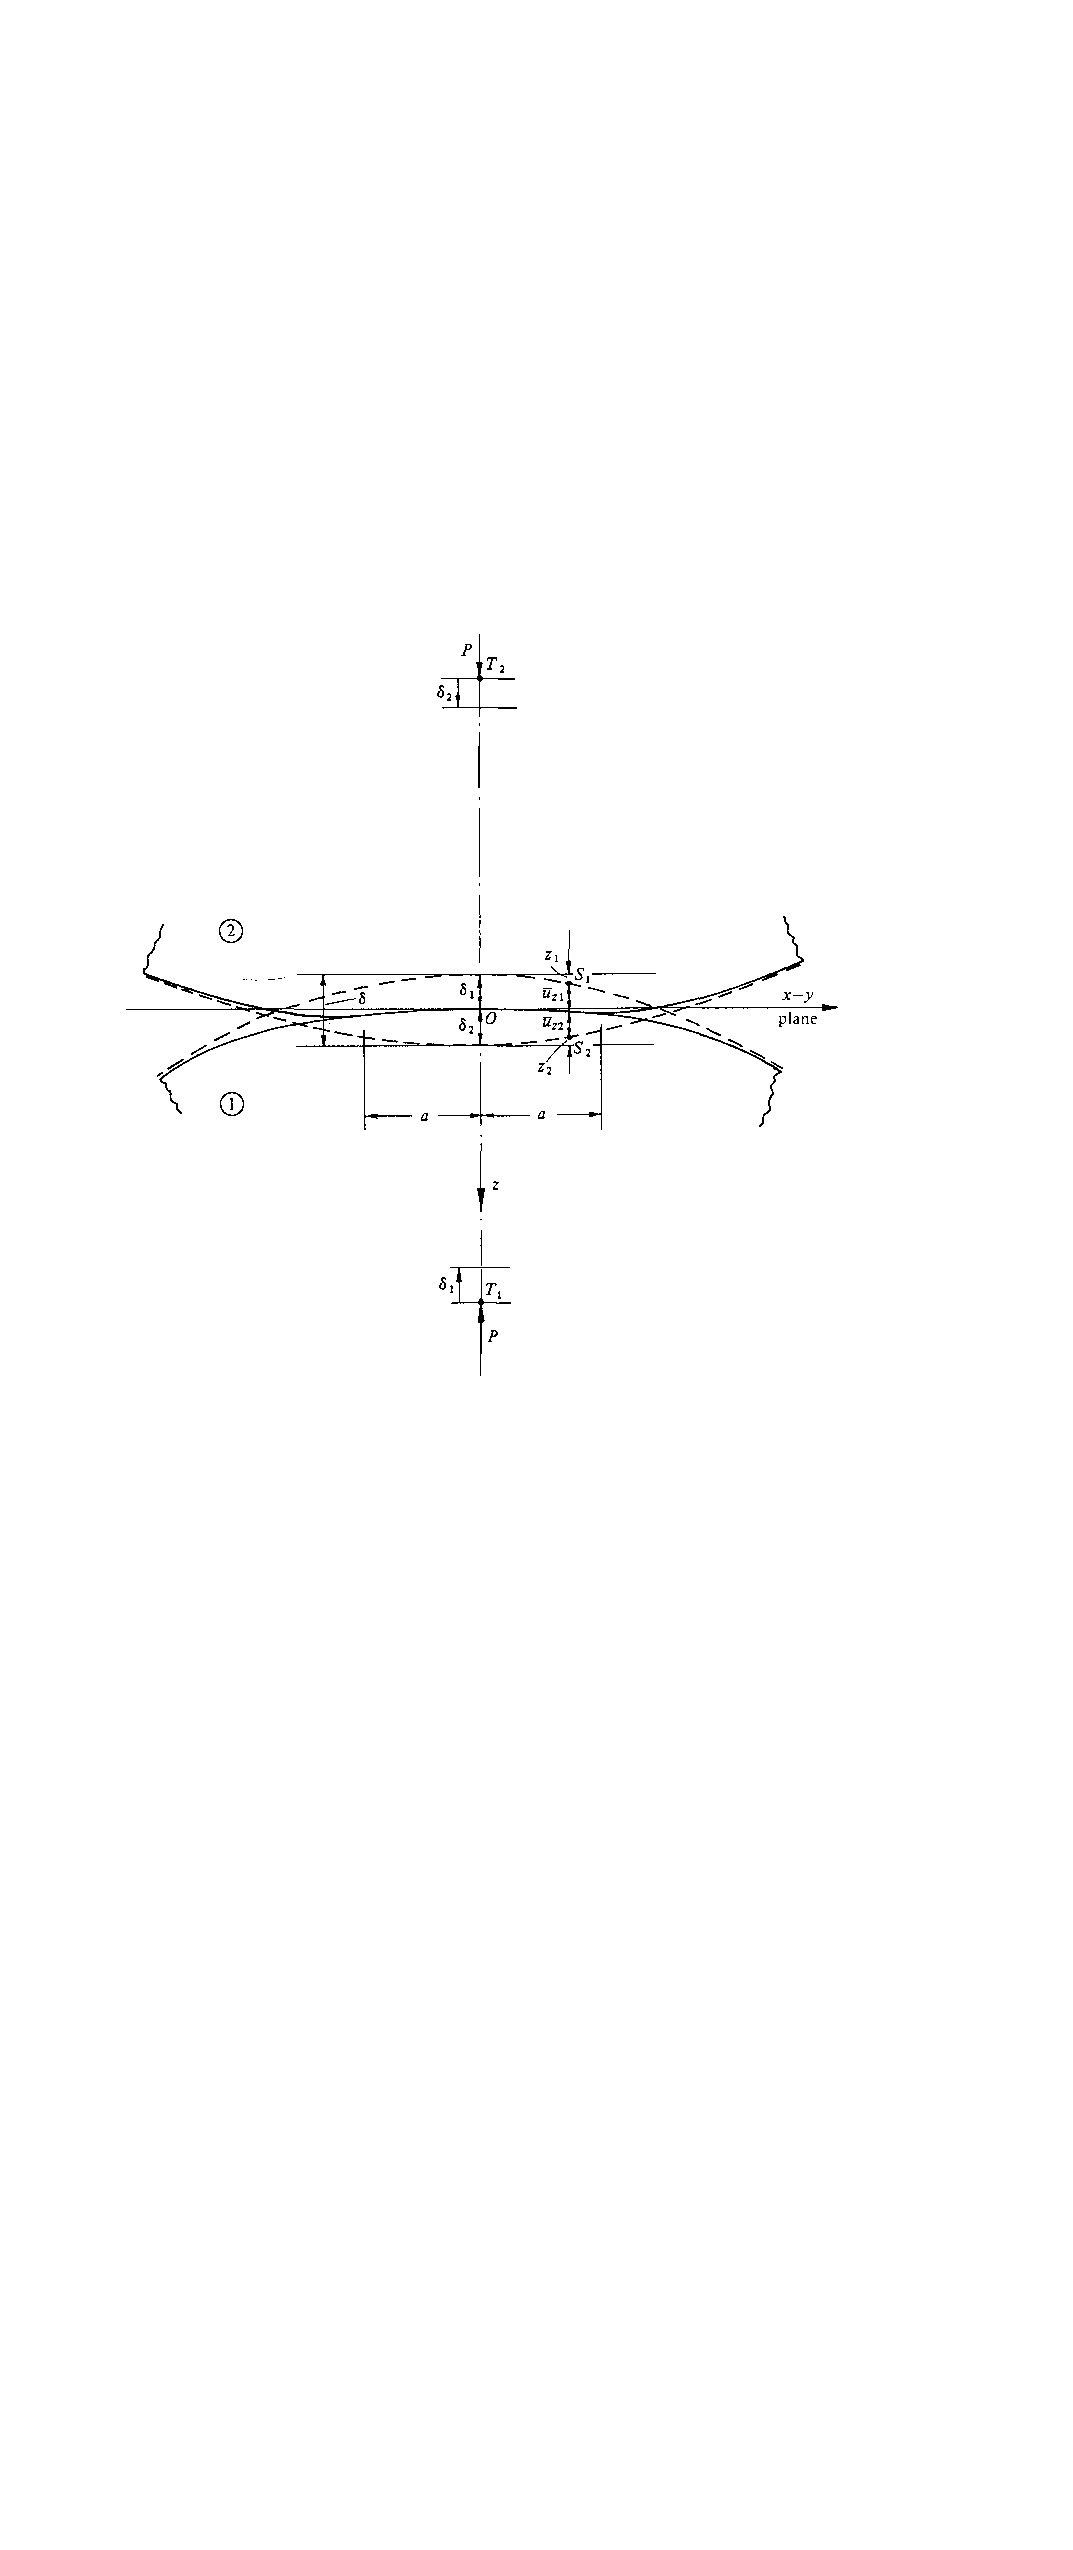
\includegraphics[width=0.85\textwidth]{chapters/figures/hertzGeometry}
	\caption{default}
	\label{fig:hertzgeometry}
	\end{center}
\end{figure}

The two bodies continue their approach towards each other until finally, under an external load $F$, come into contact. The cross-section of these bodies after contact are shown in Fig.~\ref{fig:hertzgeometry}. If we first imagine that the two surfaces do not interact and their surfaces pass through each other unimpeded, their surfaces would be overlapped to a distance $\delta$. In such a case, we examine two points deep within the bodies, along the axis of contact, calling them $T_{1}$ and $T_2$. These points will have moved $\delta_1$ and $\delta_2$, respectively. The total overlap is obviously related to these displacements by $\delta = \delta_1 + \delta_2$. 

However, under actual interaction, the two surfaces are going to deform as the load $F$ presses them into contact. So now we consider two points on the surfaces, such as $S_1$ and $S_2$. Before contact, these two points are initially are separated by a distance $h$ (from Eq.~\ref{eq:separationh}), then displace by $\bar{u}_{z1}$ and $\bar{u}_{z2}$ due to contact pressure. 

If the points $S_1$ and $S_2$ are inside of the contact region under load, these distances are related by

\begin{equation}
	\bar{u}_{z1} + \bar{u}_{z2} + h = \delta
\end{equation}

Then using Eq.~\ref{eq:separationh}, we have an expression for the elastic displacements as

\begin{equation}\label{eq:hertzdisplacements}
	\bar{u}_{z1} + \bar{u}_{z2} = \delta - \frac{1}{2R^*} \, r^2
\end{equation}

Alternatively, if after deformation the points $S_1$ and $S_2$ are outside of the contact region, this is simply

\begin{equation}\label{eq:hertz-disp-2}
	\bar{u}_{z1} + \bar{u}_{z2} > \delta - \frac{1}{2R^*} \, r^2
\end{equation}

It now is necessary to find a pressure distribution that satisfies these boundary conditions of displacement. Hertz's great contribution was to simplify the solution of expressions Eqs.~\ref{eq:hertzdisplacements} and~\ref{eq:hertz-disp-2} by regarding each body as an elastic half-space upon which the load is applied over a small, elliptical region (the contact area). This simplification allows for treatment of the highly concentrated stresses near the region of contact without consideration of either the general response of stresses in the bulk of the body or the manner in which they are supporting the load. This assumption is justifiable if the dimensions of each body as well as the relative radii of curvature are very large compared to the contact area. These assumptions are sufficient to proceed with the analysis, but the curious are pointed to an excellent discussion and background of Hertz's theory as given in KE Johnson's textbook~\cite{Johnson1985}.

For solids of revolution, a distribution of pressure to satisfy the displacements of Eq.~\ref{eq:hertz-disp-2} is proposed by Hertz as

\begin{equation}
	p = p_0 \left[1-\left(\frac{r}{a}\right)^2\right]^{1/2}
\end{equation}

where $a$ is the radius of the contact area.

The total load, $F$ is found from the pressure distribution as

\begin{align}
	F &= \int_0^a \! p(r) 2\pi r\, \mathrm{d}r \nonumber\\
	F & = \frac{2}{3} p_0 \pi a^2\label{eq:hertzforcewithpressure}
\end{align}

From the distributed load over the circular region, stresses and deflections are found from superposition of point loads. The pressure is integrated (see Ref.~\cite{Johnson1985}) to find the normal displacement for either solid body as

\begin{equation}
	\bar{u}_z = \frac{1-\nu^2}{E}\frac{\pi p_0}{4a}\left(2a^2 - r^2\right)
\end{equation}

This is applied to both bodies and plugged into Eq.~\ref{eq:hertzdisplacements} to yield

\begin{equation}\label{eq:pressindisplacement}
	\frac{\pi p_0}{4aE^*}\left(2a^2 - r^2\right) = \delta - \left(\frac{1}{2R^*}\right)\, r^2
\end{equation}

where we have introduced the now-common term of pair Young's modulus,

\begin{equation}
	\frac{1}{E^*} = \frac{1-\nu_1^2}{E_1} + \frac{1-\nu_2^2}{E_2}
\end{equation}

for simplification.

With the solution of Eq.~\ref{eq:pressindisplacement}, if we consider $r = a$ and $\delta(a) = 0$, we find the radius of the contact circle is

\begin{equation}\label{eq:hertz-radius}
	a = \frac{\pi p_0 R^*}{2E^*}
\end{equation}

and when $r= 0$, we find the overlap as

\begin{equation}
	\delta = \frac{\pi a p_0}{2E^*}
\end{equation}

and alternatively we find the pressure as a function of overlap

\begin{equation}
	p_0 = \frac{2E^*\delta}{\pi a}
\end{equation}

The radius, overlap, and pressure relations are inserted into Eq.~\ref{eq:hertzforcewithpressure} to find the force (from now on referred to as the Hertz force) as a function of overlap, relative radius, and pair Young's modulus,

\begin{equation}\label{eq:hertz-force}
	F = \frac{4}{3}E^* \sqrt{R^*} \, \delta^{3/2}
\end{equation}

as a last step, to differentiate the force from other terms to be derived later, we specify it as the normal force between sphere $i$ and sphere $j$ as

\begin{equation}\label{eq:hertz-normal-force}
	F_{n,ij} = \frac{4}{3}E_{ij}^* \sqrt{R_{ij}^*} \, \delta_{n,ij}^{3/2}
\end{equation}

Equation~\ref{eq:hertz-normal-force} defines the normal contact forces between any two contacting, elastic spheres. This extremely important result acts as the basis of all discrete element method codes since the concept was first introduced for granular materials by Cundall \& Strack in 1979\cite{Cundall1979}. 

It is very appealing to use the Hertz force in a numerical model such as DEM because there are very few assumptions built in to the theory; the material must be elastic and satisfy

\begin{equation}
	\frac{a}{R^*} \ll 1
\end{equation}

In which case the force of Eq.~\ref{eq:hertz-normal-force} is calculated from material and geometric properties alone and no phenomenological, empirical fits are necessary.



